\chapter{ANALISIS DAN PERANCANGAN}

\section{Model Desain}
    Secara garis besar, topik ini akan dibagi menjadi dua buah subsistem yang lebih kecil yakni \textit{resource allocator} dan DDS.
    Penjelasan lebih lanjut mengenai rincian desain subsistem dan pembagian kerja akan dibahas pada tabel \ref{tab:subsistemDivision}.
    \begin{table}[tbh]
        \caption{Pembagian Subsistem}\label{tab:subsistemDivision}
        \begin{center}
            \begin{tabular}{|m{0.5cm}|m{3cm}|m{5.5cm}|m{3cm}|}
                \hline
                \thead{No} & \thead{Subsistem} & \thead{Rincian Desain Subsistem} & \thead{Pembagian Kerja}\\
                \hline 
                1 & \textit{Resource Allocator} & \textit{Resource Allocator} berperan untuk melakukan alokasi \textit{bandwidth} secara tepat dan efisien yang bertujuan untuk meningkatkan rata-rata akurasi dari sistem \gls{vap} & Faishal Zharfan \\
                \hline 
                2 & DDS & DDS berperan dalam optimasi pengaturan konfigurasi parameter pengkodean dan kompresi video untuk mencapai akurasi inferensi terbaik. & Farhan Krishna\\
                \hline 
            \end{tabular}
        \end{center}
    \end{table}
    \subsection{\textit{Resource Allocator}}

    \begin{figure}[tbh]
        \centering
        \includesvg[scale=0.45]{./resources/resourceAlloc_simple.svg}
        \caption{Resource Allocator Simple}\label{fig:resourceAllocSimple}
    \end{figure}

    Secara umum, \textit{resource allocator} yang akan didesain memiliki alur kerja seperti pada gambar \ref{fig:resourceAllocSimple} di atas. 
    Terdapat 4 proses utama yakni \textit{Initialization}, \textit{Profiling}, \textit{Optimization}, dan \textit{Allocation}.
    \textit{Initialization} adalah sebuah proses ketika pertama kali \textit{resource allocator} dijalankan, pada proses ini \textit{resource allocator} akan membaca parameter-parameter yang di-sebutkan, menyiapkan port komunikasi, dan memulai \textit{worker} pada \textit{background}.
    Pada proses ini pula klien-klien akan melakukan checkin dan menjalin komunikasi dengan resource allocator menggunakan gRPC api, perilaku terakhir adalah pembagian bandwidth kepada masing-masing \gls{vap}

    \textit{Resource allocator} akan menunggu hingga proses \textit{Profiling} tiba. Proses ini akan meminta \gls{vap} yang terhubung untuk menaikan dan menurunkan \textit{bandwidth} masing-masing dan melakukan \textit{inference} terhadap \textit{bandwidth} yang bersangkutan.
    Setelahnya, hasil deteksi objek kedua \textit{bandwidth} akan diperoleh, kedua hasil ini akan dibandingkan dengan hasil deteksi objek pada \textit{bandwidth} saat ini, hasil ini lah yang dinamakan sensitivity. Sensitivity kemudian akan dikirim kepada \textit{resource allocator}
    untuk selanjutnya diproses dan dilakukan penentuan alokasi \textit{bandwidth}.

    Setibanya sensitivity pada resource allocator, proses selanjutnya adalah \textit{Optimization}. Pada proses ini, sensitivity akan diolah sedemikian sehingga tiap sensitivity menjadi sebuah persamaan garis dan dijalankan algoritma \textit{linear programming} untuk menentukan \textit{besaran bandwidth} terbaik.
    Selanjutnya hasil \textit{Optimization} akan berupa alokasi \textit{bandwidth} yang sesuai dengan kebutuhan \gls{vap}. \textit{Allocation} akan mengirimkan notifikasi kepada \gls{vap} terkait alokasi \textit{bandwidth} yang mereka dapatkan.
    Lebih lengkap terkait implementasi proses-proses tersebut akan dibahas pada bagian selanjutnya.

\section{Implementasi}
    \subsection{Initialization}

        \begin{figure}[tbh]
            \centering
            \includesvg[scale=0.5]{./resources/init.svg}
            \caption{Initialization Flow Chart}\label{fig:initialization}
        \end{figure}    

        Proses \textit{Initialization} secara umum dapat dilihat pada gambar \ref{fig:initialization}. Proses pertama yang dilakukan adalah Parameter Loading adalah membaca parameter yang terdapat pada program \textit{runResourceAllocator.sh}
        Parameter-parameter yang ada pada program ini termasuk seperti di bawah ini

        \begin{verbatim}
            bandwidth=(1500 2100 2700 3300 4500 6000 9000)
            monitorInterval=(5)
            bandwidthDelta=(50 100 150)
        \end{verbatim}

        parameter bandwidth digunakan untuk menentukan seberapa banyak bandwidth yang ingin digunakan dalam sistem, dalam kbps.
        Parameter monitorInterval menandakan periode profiling atau pengalokasian bandwidth. Parameter bandwidthDelta menandakan berapa seberapa banyak bandwidth yang ingin
        dialokasikan dari satu video ke video yang lain.

        \begin{algorithm}
        \caption{Algoritma Port Initialization}\label{alg:portInit}
        \begin{algorithmic}[1]
        \Require $workerNumber \geq 1$
        \State $srv \gets grpc.server(threadExec(workerNumber))$
        \State $srv.add\_port("0.0.0.0:5000")$
        \State $srv.start()$
        \State $srv.wait\_for\_termination()$
        \end{algorithmic}
        \end{algorithm}

        Selanjutnya adalah proses \textit{Port Initialization} yang algoritmanya dapat dilihat pada algoritma \ref{alg:portInit}. Setelah pembacaan parameter, selanjutnya 
        resource allocator akan dijalankan. Pada tahap ini algoritma memerlukan variabel workerNumber yang berguna untuk menginformasikan seberapa banyak \gls{vap} yang bisa terhubung.
        satu \gls{vap} akan memperoleh tunnel komunikasinya sendiri dengan resource allocator. Selanjutnya pada line 2, resource allocator akan dijalankan pada port 5000. Sehingga ketika 
        sebuah \gls{vap} ingin terhubung dengan resource allocator, mereka dapat menghubungi port tersebut. Lalu selanjutnya service resource allocator akan dinyalakan hingga terdapat termination.

        \begin{algorithm}[tbh]
        \caption{Algoritma App Checkin}\label{alg:appCheckin}
        \begin{algorithmic}[1]
        \Require $clientRequest$
        \Ensure $bandwidthAllocation$
        \State $NumApps \gets NumApps + 1$
        \State $bandwidthAllocation \gets MaxBW/NumApps$ \Comment{In Kbps}
        \State $app \gets PipelineRepr(clientRequest)$
        % \State $app.limit(bandwidthAllocation)$
        % \State $app.notify(bandwidthAllocation)$
        \State $clients.add(app)$
        \For{$client$ in $clients$}
        \State $client.limit(bandwidthAllocation)$
        \State $client.notify(bandwidthAllocation)$
        \EndFor
        \end{algorithmic}
        \end{algorithm}

        Selanjutnya adalah proses App checkin, pada proses ini, \gls{vap} akan melakukan check-in kepada resource allocator untuk mendapatkan alokasi bandwidth. Selain itu, \gls{vap}
        yang sudah terhubung sebelumnya akan mendapat penyesuaian jumlah bandwidth, hal ini akan terus berlangsung hingga tidak ada \gls{vap} yang melakukan check-in lagi.
        Pada kondisi saat ini, baik resource allocator dan \gls{vap} sudah saling terhubung dan dapat berkomunikasi satu sama lain.

    \subsection{Profiling}

        \begin{figure}[tbh]
            \centering
            \includesvg[scale=0.5]{./resources/profiling.svg}
            \caption{Initialization Flow Chart}\label{fig:profiling}
        \end{figure} 

        Tahapan kedua adalah \textit{Profiling}, Pada tahapan ini akan terjadi interaksi antara resource allocator dan \gls{vap}. Proses-proses yang terjadi dapat dilihat pada gambar \ref{fig:profiling}
        Pada notify client, resource allocator akan memberi notifikasi kepada \gls{vap} sebagai persiapan untuk melakukan profiling. Notifikasi yang diberika termasuk pemberian informasi mengenai seberapa
        besar delta bandwidth yang diberikan. Setelah diberikan notifikasi, \gls{vap} akan menunggu hingga inference selesai dan siap untuk proses profiling dengan memberi notifikasi kepada resource allocator.

        Hal ini berlanjut kepada proses selanjutnya yakni get inferdiff yang pseudocode nya seperti terlihat pada algoritma x di atas.


    % \begin{figure}[tbh]
    %     \centering
    %     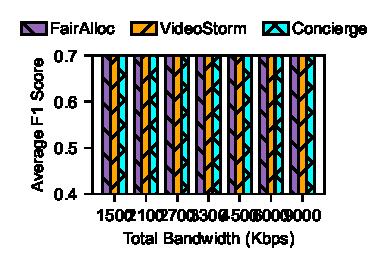
\includegraphics{./resources/concierge-perf.pdf}
    %     \caption{Tingkah Laku Sistem}\label{fig:resource_alloc_tes}
    % \end{figure}
% \begin{algorithm}
%     \caption{An algorithm with caption}\label{alg:cap}
%     \begin{algorithmic}
%     \Require $n \geq 0$
%     \Ensure $y = x^n$
%     \State $y \gets 1$
%     \State $X \gets x$
%     \State $N \gets n$
%     \While{$N \neq 0$}
%     \If{$N$ is even}
%         \State $X \gets X \times X$
%         \State $N \gets \frac{N}{2}$  \Comment{This is a comment}
%     \ElsIf{$N$ is odd}
%         \State $y \gets y \times X$
%         \State $N \gets N - 1$
%     \EndIf
%     \EndWhile
%     \end{algorithmic}
%     \end{algorithm}

